%!TEX root = ../main.tex
\begin{example}[Salary Update Error]\label{ex:telco}
  A manager updates the employees' financial records to set the tax rate to $30\%$ for high income employees who earn more than $\$87500$.
  She submits the update through a form in the salary accounting application, 
  but incorrectly types $\$85700$ for the income threshold.  
  Later queries that insert new paychecks, compute tax calculations, and
  aggregate department salaries, end up propagating this error to other records in the database, resulting in incorrect paychecks and
  employee dissatisfaction.  Figure~\ref{fig:example} illustrates this example where $Q_1$, $Q_2$, and $Q_3$ are executed on an 
  initial salary database $D_0$.  The error in the predicate of $Q_1$ is propagated to other fields in the table, by other correct queries.
\end{example}

\begin{figure}[t]
    \centering
        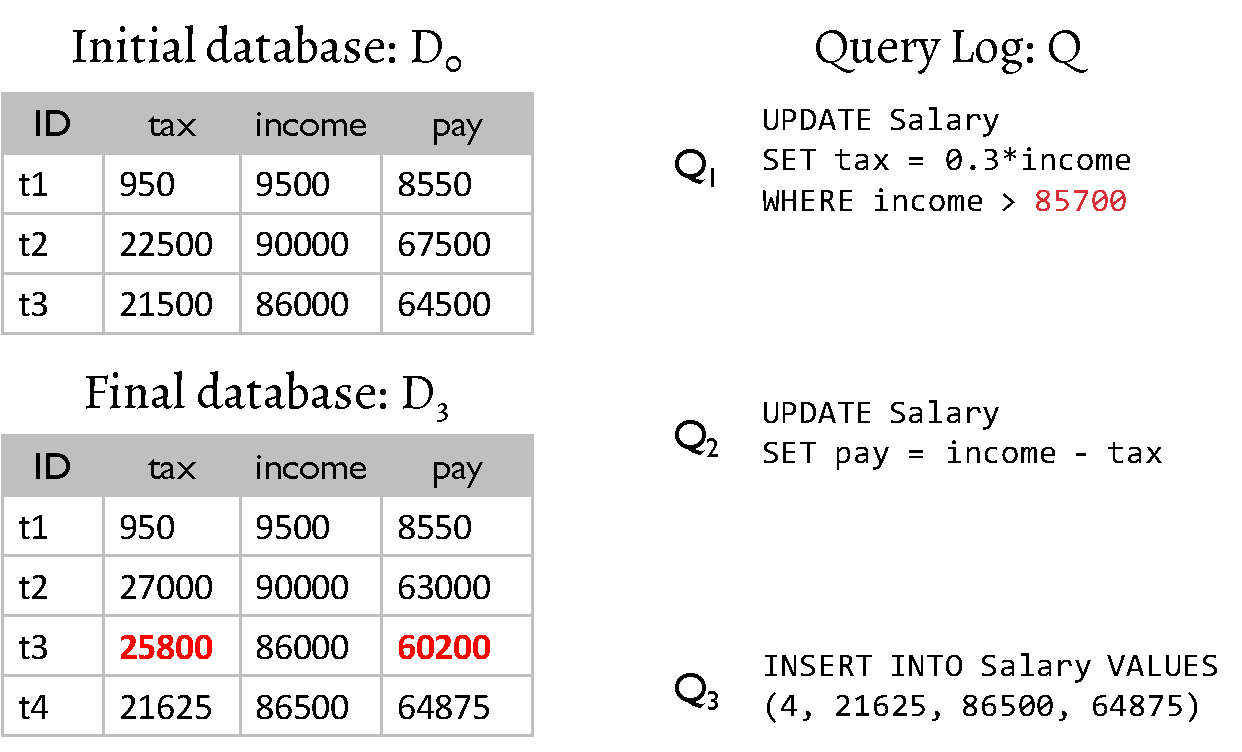
\includegraphics[width=0.4\textwidth]{figures/example2}
    \caption{\small $Q_1$ updates the tax amount with $30\%$ tax rate 
      for high income employees using an incorrect predicate.  
      The error is propogated by $Q_2$ to the $pay$ field in the database.
      Finally, a benign insert query $Q_3$ inserts correct salary information. 
      The final database state contains a mixture of incorrect and correct salary data.
    }
    \vspace*{-.2in}
    \label{fig:example}
\end{figure}


By the time some errors in the database are identified, possibly by
employees reporting incorrect paystubs, it is difficult to
(a)~identify all other errors in the database, and (b)~trace these
errors back to the erroneous update. Such problems can occur in any
data processing system with a dynamic database: errors can be
introduced by adhoc queries executed by a system administrator,
web-based forms that construct queries based on user input, stored
procedures that use human input to fill the parameter values, or even
queries with automatically generated parameters if there is a chance of
errors in the code or data used for the parameter generation.
